\pdfoutput=1
\documentclass[10pt]{beamer}

%STANDARD PREAMBLE
%https://tex.stackexchange.com/questions/68821/is-it-possible-to-create-a-latex-preamble-header
\usepackage{../../rsrc/beamer_preamble}

%% ALLOW FOR ITEMIZE ENVIRONMENTS WITH NO PRECEDING
% SPACING, IF DESIRED
% Reference: https://tex.stackexchange.com/questions/86054/how-to-remove-the-whitespace-before-itemize-enumerate
%\usepackage{enumitem}% http://ctan.org/pkg/enumitem 
\usepackage{paralist}

% RANDOM VARIABLE
\newcommand{\x}{X}
\newcommand{\y}{Y}


\title{Introduction to Maximum Likelihood Approaches}

\begin{document}

\maketitle

\begin{frame}{Table of contents}
  \setbeamertemplate{section in toc}[sections numbered]
  \tableofcontents[hideallsubsections]
\end{frame}

\begin{frame}{Acknowledgements}
This slide deck borrows heavily from an excellent course on statistical ML by Peter Orbanz.  \\
\vfill
Other useful resources came from David Blei and Michael Jordan.
\end{frame}


\section{Maximum Likelihood}

\begin{frame}{Parametric Models}

\begin{sblock}{Models}
A \bf{model} $\mathcal{P}$ is a set of probability distributions.  We index each distribution with a parameter value $\theta \in \Theta$; we can then write the model as
\[ \mathcal{P} = \set{P_\theta \cond \theta \in \Theta} \]
The set $\Theta$ is called the \bf{parameter space} of the model.
\end{sblock}

\begin{sblock}{Parametric model}
The model is called \bf{parametric} if the number of parameters (i.e. the vector $\theta$) is (1) finite and (2) independent of the number of data points.   Intuitively, the complexity of a parametric model does not increase with sample size.
\end{sblock}


\begin{sblock}{Density representation}
For parametric models, we can assume that $\Theta \subset \R^d$ for some fixed dimension $d$.   We usually represent each $P_\theta$ via a density function $p(x \cond \theta)$.
\end{sblock}
\hfill \tiny Slides in this section heavily borrow from Peter Orbanz.
\end{frame}


%%%%%%%%%%%%%%%%
\begin{frame}{Maximum Likelihood Estimation}
\begin{sblock}{Setting}
\begin{itemize}
\item Given: Data $x_1, ..., x_n$, parametric model $\mathcal{P} = \set{P_\theta \cond \theta \in \Theta}$
\item Objective: Find the distribution in $\mathcal{P}$ which best explain the data.  That means we have to choose a ``best" parameter value $\widehat{\theta}$.
\end{itemize}
\end{sblock}

\begin{sblock}{Maximum Likelihood approach}
Maximum Likelihood assumes that the data is best explained by the distribution in $\mathcal{P}$ under which it has the highest ``probability" (technically, the highest density value).

Hence, the \bf{maximum likelihood estimator} is defined as
\[ \widehat{\theta}_{\text{ML}} := \argmax_{\theta \in \Theta} p(x_1, ..., x_n \cond \theta) \]
the parameter which maximizes the joint density of the data.
\end{sblock}

\end{frame}


%%%%%%%%%%%%%%%%
\begin{frame}{The i.i.d. assumption}

\begin{sblock}{The i.i.d. assumption}
The standard assumption of ML methods is that the data is \bf{independent and identically distributed (i.i.d.)}, that is, generated by independently sampling repeatedly from the same distribution $\mathcal{P}$. 

If the density of $\mathcal{P}$ is $p(x \cond \theta)$, that means the joint density decomposes as 
\[  p(x_1, ..., x_n \cond \theta) = \ds\prod_{i=1}^n p(x_i \cond \theta) \]
\end{sblock}

\end{frame}
%SAY: Often easiest.  Give example with Poisson.  Scipy doesn't support a fit function for discrete random variables.   Statsmodels library requires specification of an "exog" variable (used for nothing), the returned parameter is nested in a table of way too much information, and if you can find it, it needs to be exponentiated. 

\begin{frame}{Illustration}
\begin{center}
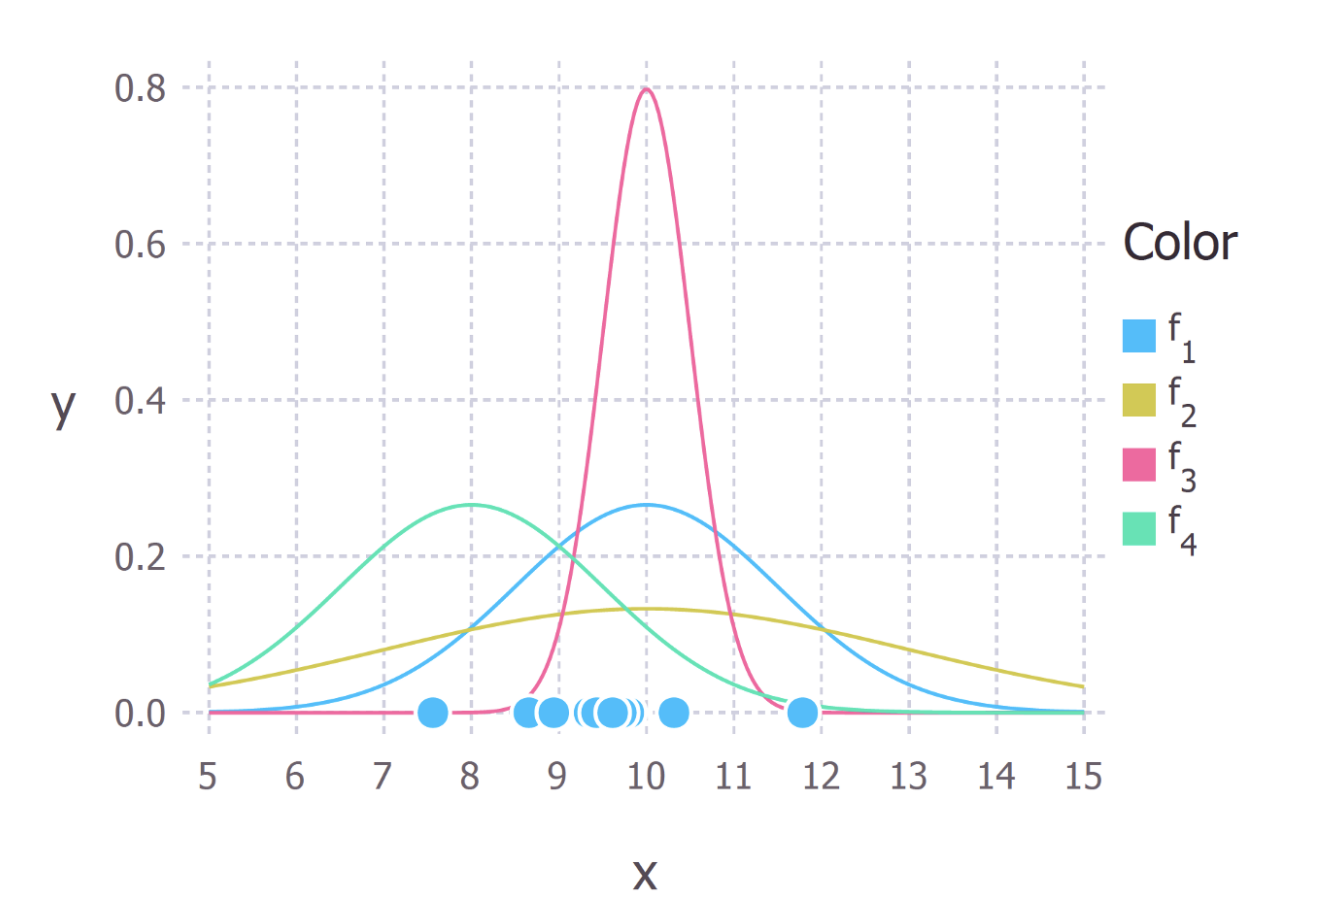
\includegraphics[width=.8\textwidth]{images/ml_example}

\vfill
\scriptsize Ten data points and four possible Gaussians from which they were drawn: $f_1 \sim \mathcal{N}(10, 2.25), f_2 \sim \mathcal{N}(10, 9), f_3 \sim \mathcal{N}(10, 0.25), f_4 \sim \mathcal{N}(8, 2.25)$.   \\ %Which distribution is the most likely to have generated the data points?
\end{center}
\hfill \tiny Image Credit: Jonny Brooks-Bartlett
% Reference https://towardsdatascience.com/probability-concepts-explained-maximum-likelihood-estimation-c7b4342fdbb1
\end{frame}


\begin{frame}{Maximum Likelihood in practice}
\begin{sblock}{Maximum Likelihood equation}
In practice, the criterion for a maximum likelihood estimator (under the i.i.d assumption) is 
\[ \nabla_\theta \bigg( \ds\prod_{i=1}^n p(x_i \cond \theta) \bigg) =0  \]
\end{sblock}
We use the ``logarithm trick" to avoid a huge product rule computation.
\end{frame}


\begin{frame}{Logarithm Trick}

\begin{sblock}{Recall: Logarithms turn products into sums}
\[ \log \bp{\ds\prod_i f_i} = \ds\sum_i  \log (f_i) \]
\end{sblock}

\begin{sblock}{Logarithms and maxima}
The logarithm is monotonically increasing on $\R_+$.\\

Consequence: Application of log does not change the \it{location} of a maximum or minimum:

\begin{align*}
\max_y \log (g(y)) &\neq \max_y g(y)  && \text{The \it{value} changes.} \\
\argmax_y \log (g(y)) &= \argmax_y g(y)  && \text{The \it{location} does not change.}
\end{align*}


\end{sblock}


\end{frame}


\begin{frame}{Maximum Likelihood in practice}


\begin{sblock}{Likelihood and logarithm trick}
\[  \widehat{\theta}_{\text{ML}} = \argmax_\theta \ds\prod_{i=1}^n p(x_i | \theta) = \argmax_\theta \log \bp{ \ds\prod_{i=1}^n p(x_i | \theta)} = \argmax_\theta \ds\sum_{i=1}^n \log p(x_i | \theta)  \]
\end{sblock}

\begin{sblock}{Maximum Likelihood in practice (revisited)}

\[ 0 = \ds\sum_{i=1}^n \nabla_\theta \log p(x_i | \theta) = \ds\sum_{i=1}^n \df{\nabla_\theta p(x_i |\theta) }{p(x_i |\theta)} \]

Whether or not we can solve this analytically depends on the choice of model!
\end{sblock}

\end{frame}


\section{Maximum Likelihood Examples}

\begin{frame}{Example: Gaussian Distribution}

\begin{sblock}{Gaussian density in one dimension}
\begin{columns}
\begin{column}{.55\textwidth}
\footnotesize
\[ g(x; \mu, \sigma) := \df{1}{\sqrt{2 \pi} \sigma} \exp \bp{ - \df{(x-\mu)^2}{2 \sigma^2}} \]
\begin{compactitem}
\item $\mu$ = expected value of $x$, $\sigma^2$ = variance, $\sigma$ =  standard deviation
\item The quotient $\frac{x - \mu}{\sigma}$ measures deviation of $x$ from its expected value in units of $\sigma$ (i.e., $\sigma$ defines the length scale).
\end{compactitem}
\end{column}
\begin{column}{.3\textwidth}
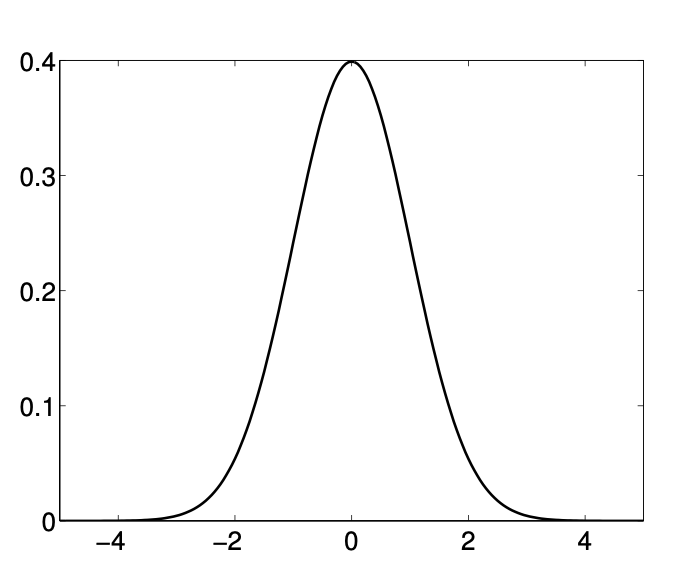
\includegraphics[width=\textwidth]{images/gaussian_1d}
\end{column}
\end{columns}
\end{sblock}

\begin{sblock}{Gaussian density in $d$ dimensions}
\begin{columns}
\begin{column}{.55\textwidth}
\footnotesize
\vfill \vfill \vfill
The quadratic function 
\[ - \df{(x-\mu)^2}{2 \sigma^2} = -\df{1}{2} (x-\mu) (\sigma^1)^{-1} (x - \mu) \]
is replaced by a quadratic form:
\[ g(\+x; \+\mu, \Sigma) := \df{1}{\sqrt{2 \pi |\Sigma|}} \exp \bp{ - \df{1}{2} (\+x - \+\mu)^T \Sigma^{-1} ( \+x - \+\mu)} \]
\end{column}
\begin{column}{.3\textwidth}
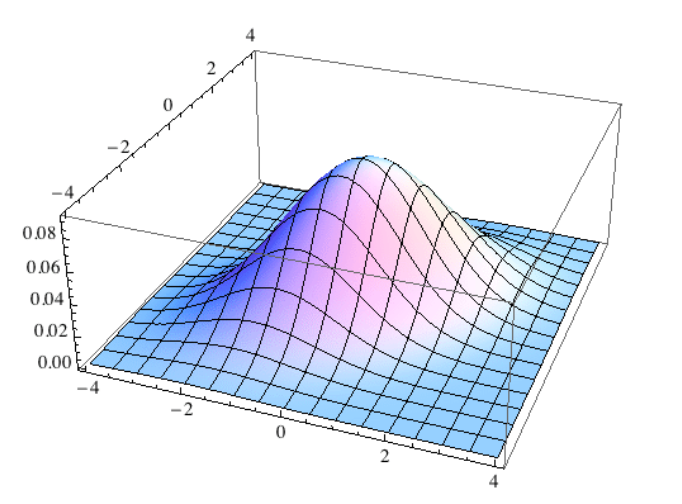
\includegraphics[width=\textwidth]{images/gaussian_nd}
\end{column}
\end{columns}
\end{sblock}

\end{frame}



\begin{frame}{Example: Gaussian Mean MLE}

\begin{sblock}{Model: Multivariate Gausians}
The model $\mathcal{P}$ is the set of all Gaussian densities on $\R^d$ with \textit{fixed} covariance matrix $\Sigma$
\[ \mathcal{P} = \set{g(\cdot \cond \mu, \Sigma) \cond \mu \in \R^d} \]
where $g$ is the Gaussian density function.  The parameter space is $\Theta = \R^d$.
\end{sblock}

\begin{sblock}{MLE equation}

We have to solve the maximum likelihood equation 
\[ \ds\sum_{i=1}^n \nabla_\mu \log g(x_i \cond \mu, \Sigma) = 0 \]
for $\mu$.
\end{sblock}

\end{frame}


\begin{frame}{Example: Gaussian Mean MLE}
\footnotesize
\begin{align*}
0 &= \ds\sum_{i=1}^n  \nabla_\mu  \log \bb{\df{1}{\sqrt{(2 \pi)^d |\Sigma| }} \exp \bp{ - \df{1}{2} (\+x - \+\mu)^T \Sigma^{-1} ( \+x - \+\mu)}}   \\
&=  \ds\sum_{i=1}^n   \nabla_\mu  \bb{\log \df{1}{\sqrt{(2 \pi)^d |\Sigma| }}} +\nabla_\mu \bb{ \log \bp{\exp \bp{ - \df{1}{2} (\+x - \+\mu)^T \Sigma^{-1} ( \+x - \+\mu)} }} \\
&=  \ds\sum_{i=1}^n \nabla_\mu \bp{ - \df{1}{2} (\+x - \+\mu)^T \Sigma^{-1} ( \+x - \+\mu)}  = -  \ds\sum_{i=1}^n \Sigma^{-1} (x_i - \+\mu) 
\end{align*}

Multiplication by $(- \Sigma)$ gives

\[  0 = \ds\sum_{i=1}^n (x_i - \+\mu) \implies \+\mu = \df{1}{n} \ds\sum_{i=1}^n x_i\]

\begin{sblock}{Conclusion}
The maximum likelihood estimator of the Gaussian expectation parameter for fixed covariance is 
\[ \widehat{\+\mu}_{\text{ML}} := \df{1}{n} \ds\sum_{i=1}^n x_i \]
\end{sblock}

\end{frame}


\begin{frame}{Example: Gaussian with Unknown Mean, Covariance}
\footnotesize
\begin{sblock}{Model: Multivariate Gaussians}
The model $\mathcal{P}$ is now
\[ \mathcal{P} = \set{g(\cdot \cond \mu, \Sigma) \cond \mu \in \R^d, \Sigma \in \Delta_d} \]
where $\Delta_d$ is the set of postive definite $d \times d$-matrices. The parameter space is $\Theta = \R^d \times \Delta_d$.
\end{sblock}

\begin{sblock}{ML approach}
Since we have just seen that the ML estimator of $\mu$ does not depend on $\Sigma$, we can compute $\widehat{\+\mu}_\text{ML}$ first. We then estimate $\Sigma$ using the criterion

\[ \ds\sum_{i=1}^n \nabla_\Sigma \log g(x_i \cond \widehat{\+\mu}_\text{ML}, \Sigma) = 0 \]
for $\mu$.
\end{sblock}

\begin{sblock}{Solution}
The ML estimator of $\Sigma$ is 

\[  \widehat{\Sigma}_\text{ML} = \df{1}{n} \ds\sum_{i=1}^n (x_i -  \widehat{\mu}_\text{ML}) (x_i - \widehat{\mu}_\text{ML})^T \]
for $\mu$.
\end{sblock}

\end{frame}

\begin{frame}{Exercises}

Let's split into break-out rooms and try some \href{https://colab.research.google.com/drive/1aNNOV0fdAcDiKKKGp5dodGtEA5sk96TH}{\blue{ML exercises}}

\end{frame}



\section{Anomaly Detection with Multivariate Gaussians}

\begin{frame}{Anomaly Detection with Multivariate Gaussians}

Given a fitted Gaussian model, how can we assess the anomalousness of test data?

\pause 
\begin{center}
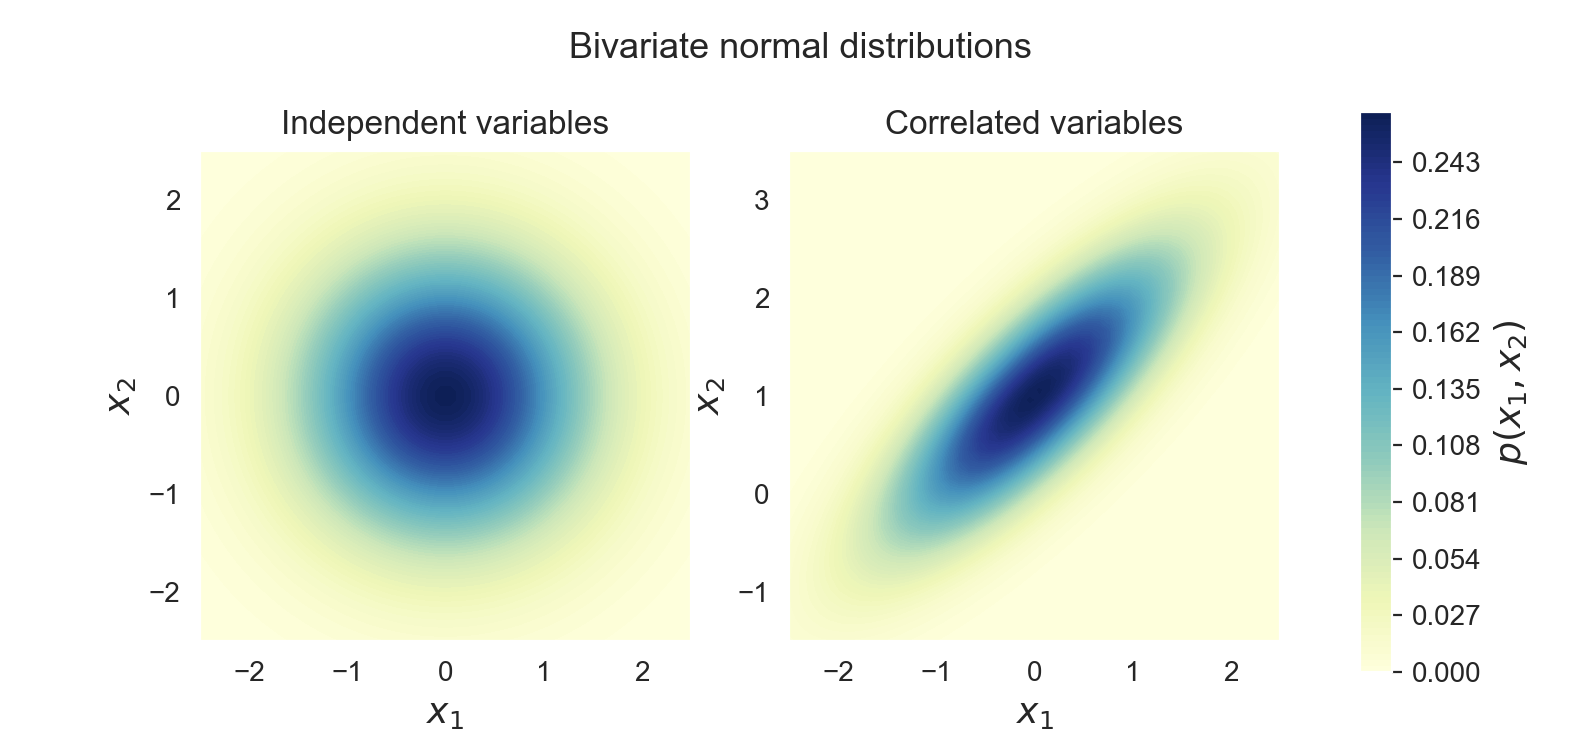
\includegraphics[width=.6\textwidth]{images/gaussian_heatmap_independent_correlated}
\end{center}

\vfill
\hfill \tiny Image Credit: Peter Roelants
\pause

\begin{sblock}{Mahalanobis Distance}
\footnotesize
For a Gaussian random variable $X \sim N (\+\mu, \Sigma)$,  the quadratic form (or \it{squared Mahalanobis distance}) has known distribution 

\[ \Delta^2 = (\+X - \+\mu) ^T \Sigma^{-1} (\+X - \+\mu) \sim \chi^2(d) \]

This can be used to assess the anomalousness of test data.
\end{sblock}
% SAY:  Note from the density that these are equi-probability contours 

\end{frame}

\begin{frame}{Exercises}

Let's split into break-out rooms and try some \href{https://colab.research.google.com/drive/1tqG8H1m5TyBwtK_Rdnh9uYWMjzvJySvy}{\blue{exercises}}

\end{frame}



\section{Optimization}

\begin{frame}{Optimization problem}
An \textit{optimization problem} for a given function $f : \R^d \to \R$ is a problem of the form 
\[ \min_{\+x} f (\+x) \]
which we read as ``find $\+x_0 = \arg\min_{\+x} f (\+x)$'''. 
\vfill
Note that finding the maximum likelihood requires minimizing the cost function that is the negative log likelihood.

\end{frame}

\begin{frame}{Local and global modes}

\begin{center}
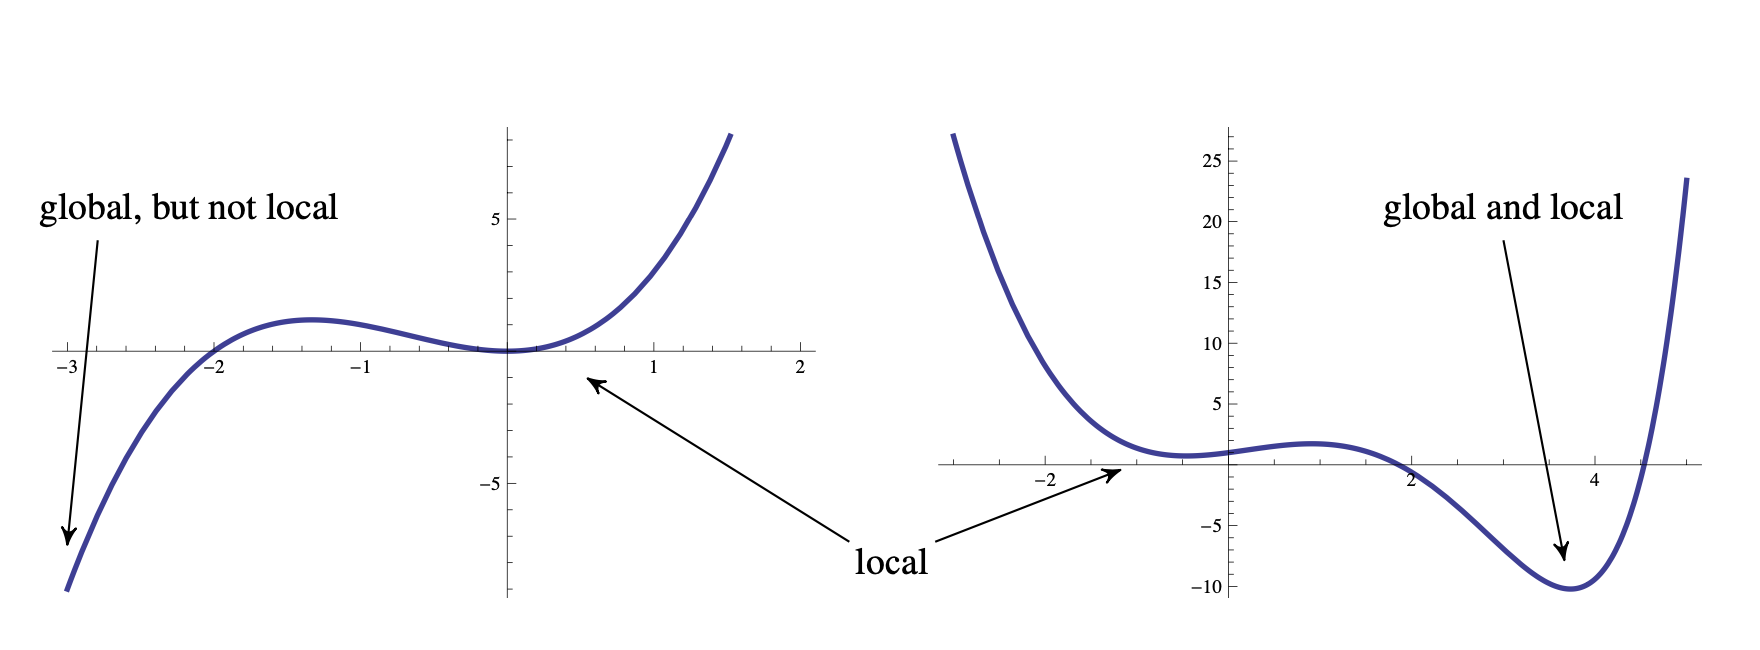
\includegraphics[width=.8\textwidth]{images/types_of_minima}
\end{center}


\begin{sblock}{Local and global minima}
A minimum of a function $f$ at $x$ is called
\begin{itemize}
\item \bf{Global} if $f$ assumes no smaller value on its domain.
\item \bf{Local} if there is some open neighborhood $U$ of $x$ such that $f(x)$ is a global minimum of $f$ restricted to $U$.
\end{itemize}
\end{sblock}
\tiny \hfill Image Credit: Peter Orbanz
\end{frame}
% SAY: In opening: You may have noticed that we only checked for local 
% SAY: Will be important when we discuss EM, VI, and NF.


\begin{frame}{Analytic Maximum Likelihood}



\begin{sblock}{Analytic criteria for local minima}
Recall that $\+x$ is a local minimum of $f$ if
\[ f^\prime(\+x) = 0 \quad \text{and} \quad  f^{\prime \prime}(\+x) > 0  \]
In $\R^d$,

\[ \nabla f (\+x)  = 0 \; \text{and} \; H_f (\+x) = \bp{\df{\delta f}{\delta  x_i  \delta x_j}  (\+x) }_{ i,j= 1,...,n}   \; \text{positive definite} \]  
The $d \times  d$-matrix $H_f (\+x)$ is called the \bf{Hessian matrix} of $f$ at $\+x$.
\end{sblock}

\end{frame}

\begin{frame}{The MLE and Global Maximizers}

You may have noticed that the maximum likelihood equation is only tracking a \it{local} maximality criterion.  In fact, it also ignored the second-order condition. What gives?

\begin{itemize}
\item Many well-known distributions\footnote{In particular, those in the exponential family.  See the next slide.} have strictly concave likelihoods\, in which case the MLE equation is sufficient to verify a global maximum. 
\item For many other distributions, it can be hard to find the global maximizer of the likelihood. Thus a local maximizer is often used and is called an MLE.   The local optimizer is typically found by an optimization procedure, from which the second order condition generally follows.
\end{itemize}

\end{frame}

\begin{frame}{Convex Functions}

\begin{sblock}{Definitions}

\begin{minipage}{.6\textwidth}
A function $f$ is \bf{convex} if every line segment between function values lies above the graph of $f$.  \tiny{(A function $f$ is \bf{concave} if $-f$ is convex.  Some likelihood functions $L$ are \it{concave}, in which case the \it{cost function} that we want to minimize, $-L$, is convex.)}
\end{minipage}
\hfill
\begin{minipage}{.3\textwidth}
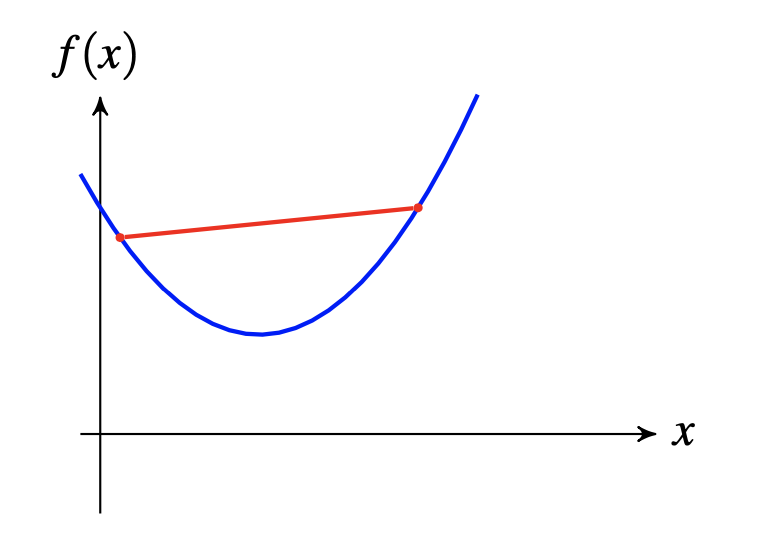
\includegraphics[width=\textwidth]{images/convexity}
\end{minipage}
\end{sblock}

\begin{sblock}{Analytic criterion}
 A twice differentiable function is convex if $f^{\prime \prime}(\+x) \geq 0$ (or $H_f (\+x)$ positive semidefinite) for all $\+x$.
\end{sblock}  
  
\begin{sblock}{Implications for optimization}
If $f$ is convex, then:
\begin{itemize}
\item $f^\prime (\+x) = 0$ is a sufficient criterion for a minimum. 
\item Local minima are global.
\item If f is strictly convex ($f^{\prime \prime} > 0$ or $H_f$ positive definite), there is only one minimum (which is both global and local).
\end{itemize}
\end{sblock}

\end{frame}

\begin{frame}{Demo}
\begin{center}
\href{https://colab.research.google.com/drive/1PokSTCC1u0QWghxLVWhS30ycVRWjNMbG}{Gradient Ascent Demo}
\end{center}
\end{frame}

\section{Exponential Family}


\begin{frame}{Exponential Family Models}

\begin{sblock}{Definition}
We consider a model $\mathcal{P}$ for data in a sample space $\mathcal{X}$ with parameter space $\Theta \subset \R^m$ . Each distribution in $\mathcal{P}$ has density $p(x \cond \theta)$ for some $\theta \in \Theta$ . \\
\vfill
The model is called an \bf{exponential family model} (EFM) if $p$ can be written as
\begin{align*}
%\label{eqn:exponential_family}
 p(x \cond \theta) = h(x) \exp \{ \eta(\theta)^T s(x) - a(\theta)\} 
 \end{align*}
where we refer to 
\begin{itemize}
\item $h$ as the base measure
\item  $\eta$ as the natural parameter
\item $s$ as the sufficient statistics
\item $a$ as the log normalizer. 
\end{itemize}
\end{sblock}
\end{frame}


\begin{frame}
\begin{sblock}{Exponential families are important because}
\begin{itemize}
\item Many important parametric models (Gaussian, Poisson, beta, gamma, etc.) are EFM's.
\item The special form of $p$ gives them many nice properties. For example, exponential family likelihoods are \it{strictly concave.}\footnote{We have seen this earlier. Other useful properties -- such as conjugacy -- will come up as we go along.}
\item Many algorithms and methods can be formulated generically for all EFM's. 
\end{itemize}
\end{sblock}
\vfill
\begin{sblock}{An observation}
The data and the parameter interact only through the linear term $\eta(\theta)^T s(x)$ in the exponent.
\end{sblock}

%
%The exponential family of distributions includes the Gaussian, binomial, multinomial, Poisson, gamma, von Mises and beta distributions, as well as many others. 
%
%Facts about the exponential family can be used to simplify many problems in machine learning.  (We have already seen one of many examples.)
\end{frame}




\begin{frame}{Example: The Gaussian distribution}
\footnotesize
The familiar form of the univariate Gaussian is 
\[ p(x \cond \mu, \sigma^2) = \df{1}{\sqrt{2 \pi \sigma^2}} \; \exp \bp{ - \df{1}{2} \df{(x-\mu)^2}{\sigma^2}}  \] 
\pause

We put it in exponential family form by expanding the square
\begin{align*}
 p(x \cond \mu, \sigma^2) = \df{1}{\sqrt{2 \pi}} \exp \bp{ \df{\mu}{\sigma^2} x - \df{1}{2 \sigma^2} x^2 - \df{1}{2 \sigma^2} \mu^2 - \log \sigma}
 \end{align*}
 which reveals the exponential family where
 \begin{align*}
\eta &= [\mu/\sigma^2, -1/2 \sigma^2 ]\\
s(x) &= [x, x^2] \\
a(\eta) &= \mu^2/2\sigma^2 + \log \sigma \\
h(x) &=  1/\sqrt{2 \pi}
 \end{align*}

\end{frame}


\begin{frame}{Example: The Bernoulli distribution}
\footnotesize
As an example, let's put the Bernoulli (in its usual form) into exponential family form.   The Bernoulli you are used to seeing is:
\[ p(x \cond \pi) = \pi^x \; (1-\pi)^{1-x} \quad x \in \set{0,1} \] 
\pause
In exponential family form:
\begin{align*}
 p(x \cond \pi) &= \exp \bp{  \log \bb{\pi^x \; (1-\pi)^{1-x} }} \\
 &= \exp \bp{ x \log \pi + (1-x) \log (1-\pi)} \\
 &= \exp \bp{x \log \pi - x \log (1-\pi) + \log (1-\pi)} \\
&= \exp \bp{x \log (\pi/(1-\pi)) + \log (1-\pi) } 
 \end{align*}
 which reveals the exponential family where
 \begin{align*}
\eta &= \log(\pi / (1-\pi) ) \\
s(x) &= x\\
a(\eta) &= -\log (1-\pi) = \log (1 + e^\eta) \\
h(x) &=  1
 \end{align*}
\noindent\rule{2cm}{.4pt} \\
\tiny  Note that the relationship between $\pi$ and $\eta$ is invertible
\[ \pi = 1/(1 + e^{-\eta})\] 
 This it the \it{logistic function}.


\end{frame}


\begin{frame}{Example: The Dirichlet Distribution}


\begin{columns}
\begin{column}{.6\textwidth}
We can write the density of the Dirichlet distribution in exponential form:
\end{column}
\begin{column}{.35\textwidth}
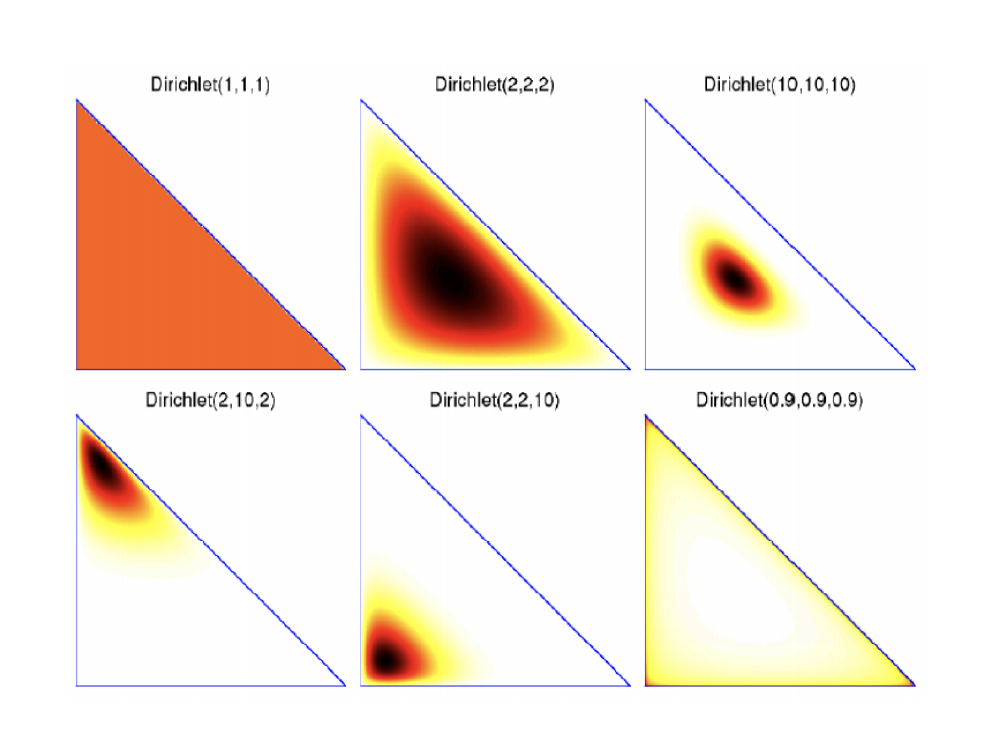
\includegraphics[width=\textwidth]{images/dirichlet}
\end{column}
\end{columns}
\begin{align*}
p (\pi \cond\alpha) &= \df{\Gamma(\sum_k \alpha_k)}{\prod_k \Gamma (\alpha_k) } \pi_1^{\alpha_1 -1} \cdot \cdot \cdot \pi_K^{\alpha_K -1} \\
&= \exp \bigg\{ \sum_{k=1}^K (\alpha_k -1) \log \pi_k - \bigg[ \sum_k \log \Gamma (\alpha_k)-  \log \Gamma (\sum \alpha_k) \bigg]  \bigg\}
\end{align*}
with natural parameter $\eta(\alpha) = [\alpha_1 -1, ..., \alpha_K -1]^T$, sufficient statistics $s(\pi) = \log \pi = [\log \pi_1, ..., \log \pi_K]^T$, base measure $h(\pi)=1$, and log normalizer $a(\alpha) =  \sum_k \log \Gamma (\alpha_k ) - \log \Gamma (\sum_k \alpha_k)$. $\qed$
\end{frame}



\begin{frame}{Examples of Exponential Families}
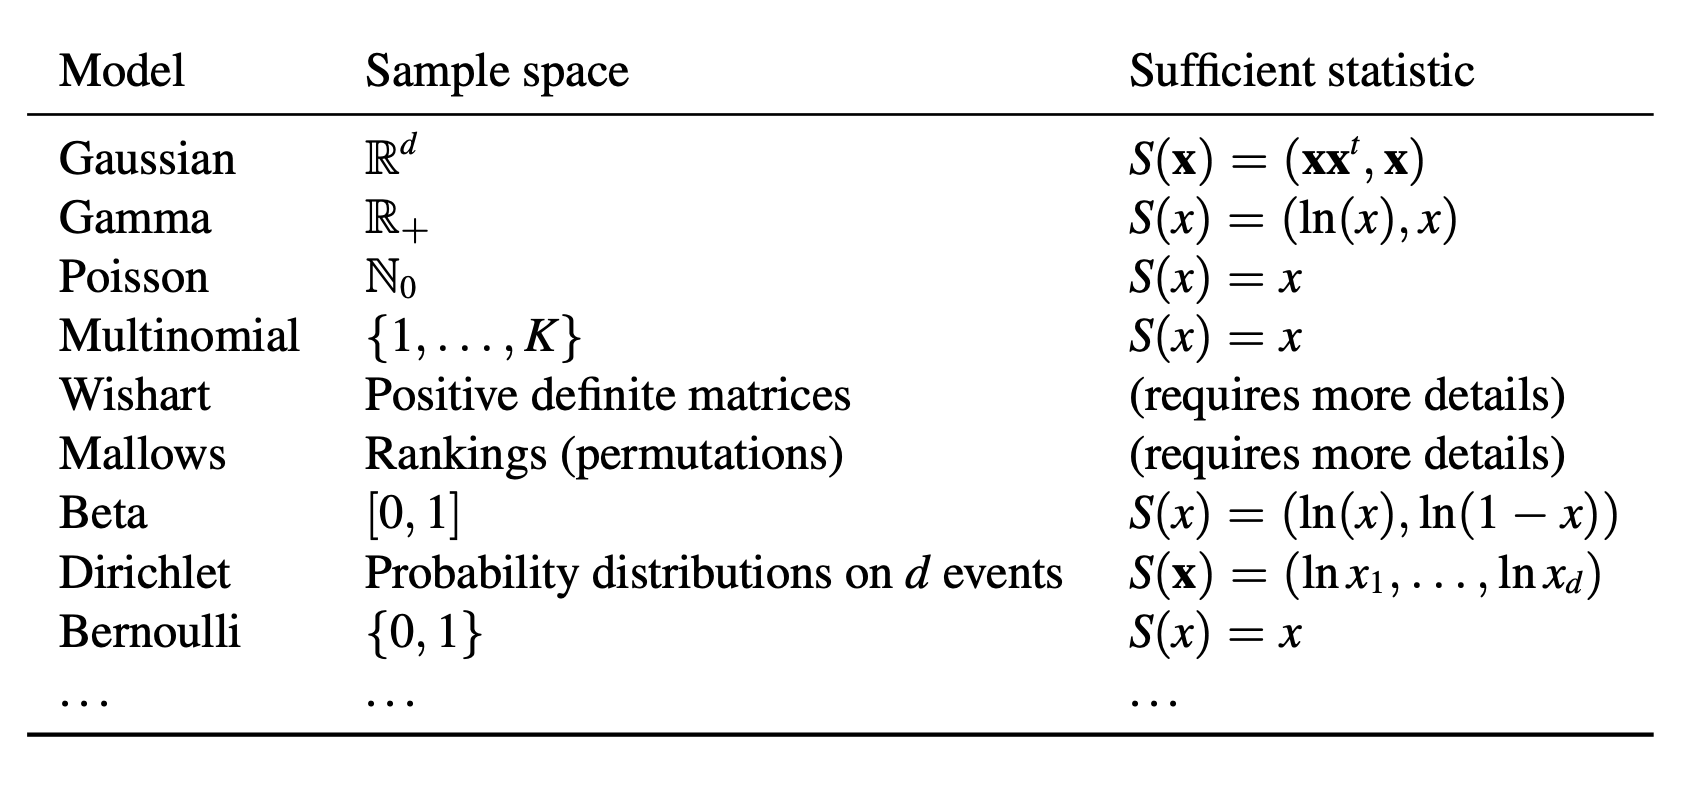
\includegraphics[width=\textwidth]{images/ef_examples}

%\hfill \tiny Image Credit: Peter Orbanz 
\begin{sblock}{Roughly speaking}
On every sample space, there is a ``natural" statistic of interest. On a space with Euclidean distance, for example, it is natural to measure both location and correlation; on categories (which have no "distance" from each other), it is more natural to measure only expected numbers of counts. %On most types of sample spaces, the exponential family model with S chosen as this natural statistic is the prototypical distribution
\end{sblock}



\end{frame}



\begin{frame}{The Exponential Family and Maximum Likelihood}
\begin{sblock}{i.i.d samples from an exponential family distribution}
If $\+x=(x_1, ..., x_n)$ are n independent samples from the same exponential family distribution, then 
\begin{align*}
%\label{eqn:exponential_family_iid}
 p(\+x \cond \theta) = \ds\prod_{i=1}^n h(x_i) \exp \big\{ \eta(\theta)^T \sum_{i=1}^n s(x_i) - n \,a(\eta(\theta))\big\} 
 \end{align*}
 \end{sblock}
 
 \begin{sblock}{Maximum likelihood with exponential families}
 The goal for maximum likelihood is to determine parameter
\begin{equation*}
%\label{eqn:ml}
\theta_{ML} = \argmax_\theta  \, \log p(\+x \cond \theta) 
\end{equation*}

Let us assume that $\+x=(x_1, ..., x_n)$ are i.i.d observations  from a fixed exponential family, so that the likelihood has form above.
\end{sblock}
\end{frame}

\begin{frame}{The Exponential Family and Maximum Likelihood}
\footnotesize
 Let us compute the gradient with respect to the natural parameter $\eta$ of $\ell(\eta) := \log p(\+x \cond \eta)$

\[ \nabla_\eta \ell(\eta) = \ds\sum_{i=1}^n s(x_i) - n \; \nabla_\eta a(\eta) \]

Setting the gradient to zero, we obtain

\[ \nabla_\eta a(\eta) = \df{1}{n}  \ds\sum_{i=1}^n s(x_i) \]

But\footnote{A useful fact about exponential families.  The proof is straightforward.}    $\nabla_\eta a(\eta) = \E [s(X)]$. Thus, we should set $\theta_{ML}$ such that

\[ \mu(\theta_{ML}) = \df{1}{n} \ds\sum_{i=1}^n s(x_i) \]
where $\mu := \E[s(x)]$ refers to the mean parametrization of the likelihood.
\end{frame}






\end{document}